
\section{Central tracking}

\subsection{Silicon microstrip tracker}

%%%%%% SLIDE
\begin{frame}{\textcolor{Goldenrod}{Central Tracker}}
  \begin{overlayarea}{\textwidth}{\textheight}
    \begin{figure}[h]
      \centering
      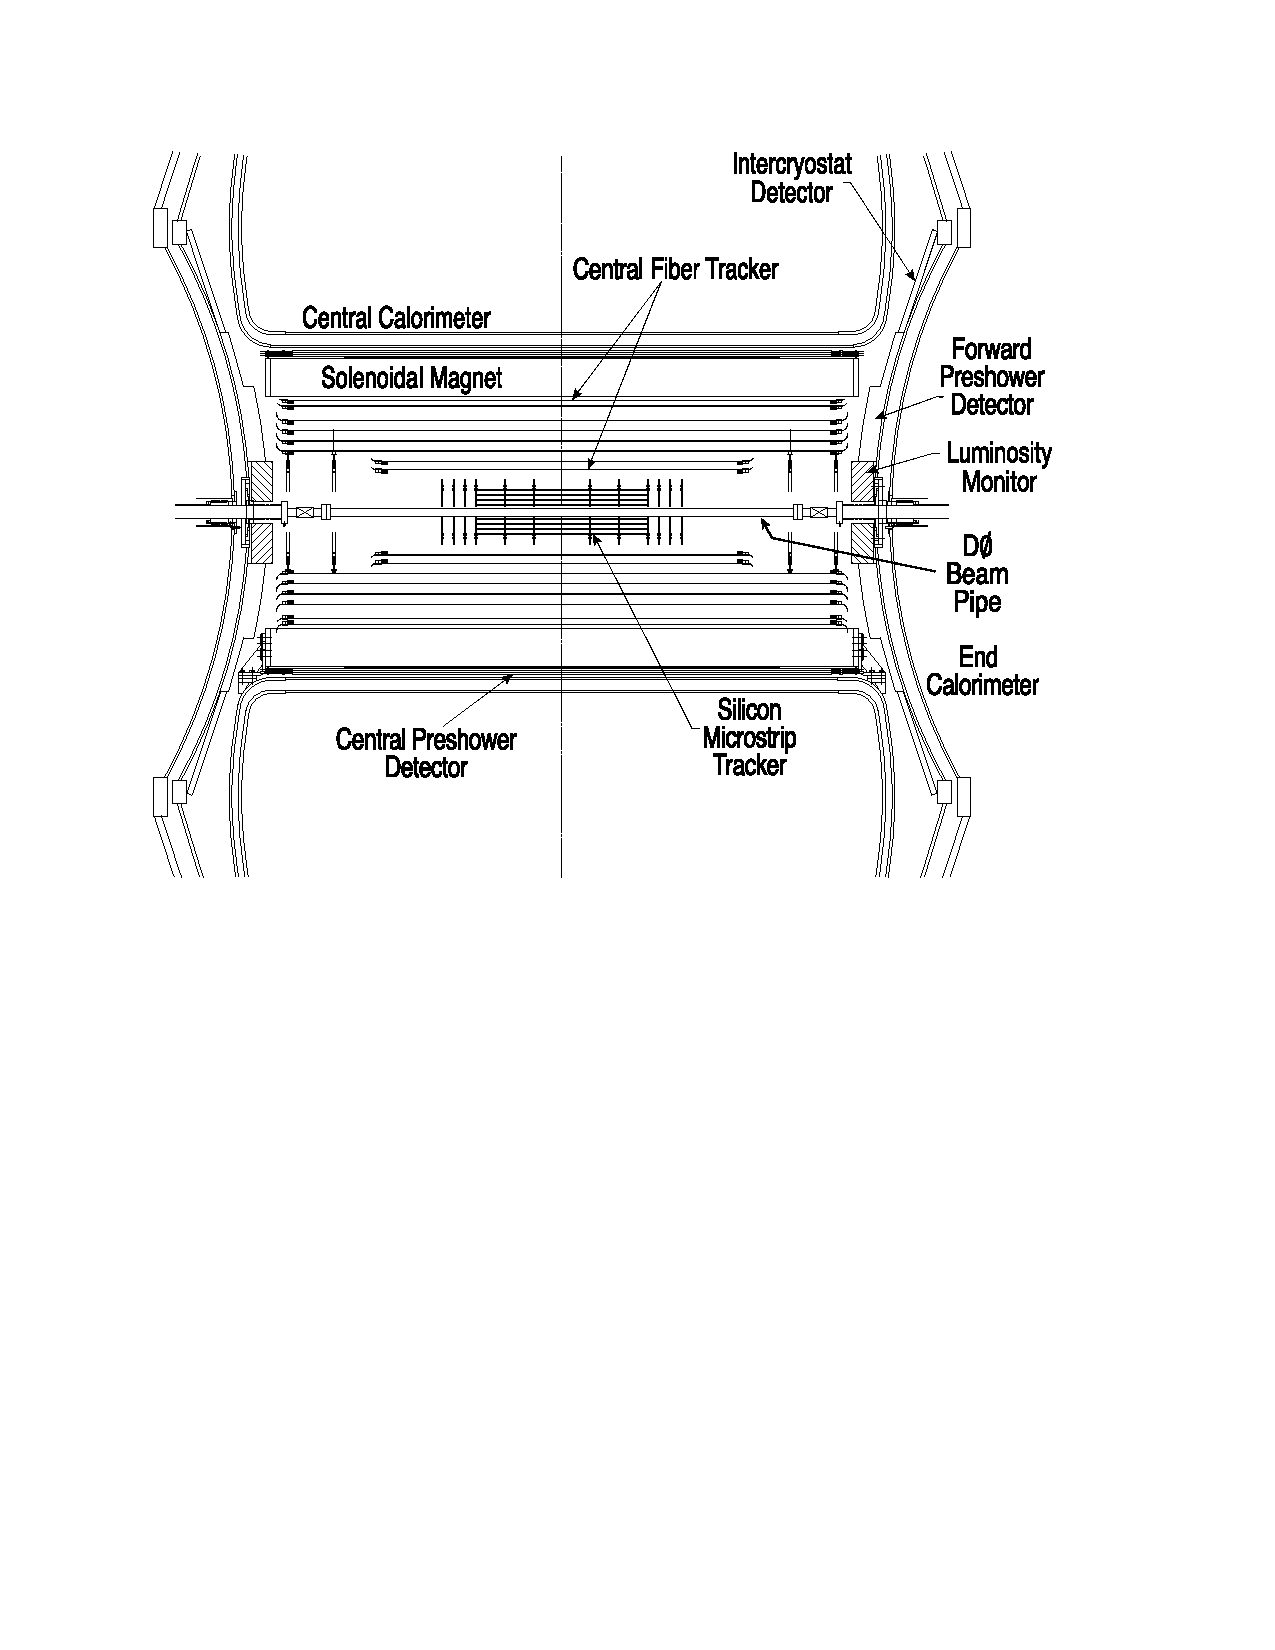
\includegraphics[height=0.4\textheight]{./Images/08_CT.pdf}
    \end{figure}
    
    \itt[<+->]
  \item
    A Silicon Microstrip Tracker (SMT) and a Central Fiber Tracker
    (CFT) within a solenoidal magnet
  \item Excellent resolution; $\sigma_{d_0} \approx 15 \mu m, 
    \sigma_{z_0}\approx 35\mu m$:\\
    \hlt{Magenta}{good $p^{lep/jet}_{T} $ and $\slashed{E_T}$ measurement}
    \tti
  \end{overlayarea}
\end{frame}


%%%%%% SLIDE
\begin{frame}{\textcolor{Goldenrod}{Silicon Microstrip Tracker}}
  \begin{overlayarea}{\textwidth}{\textheight}
    \begin{figure}[h]\centering
      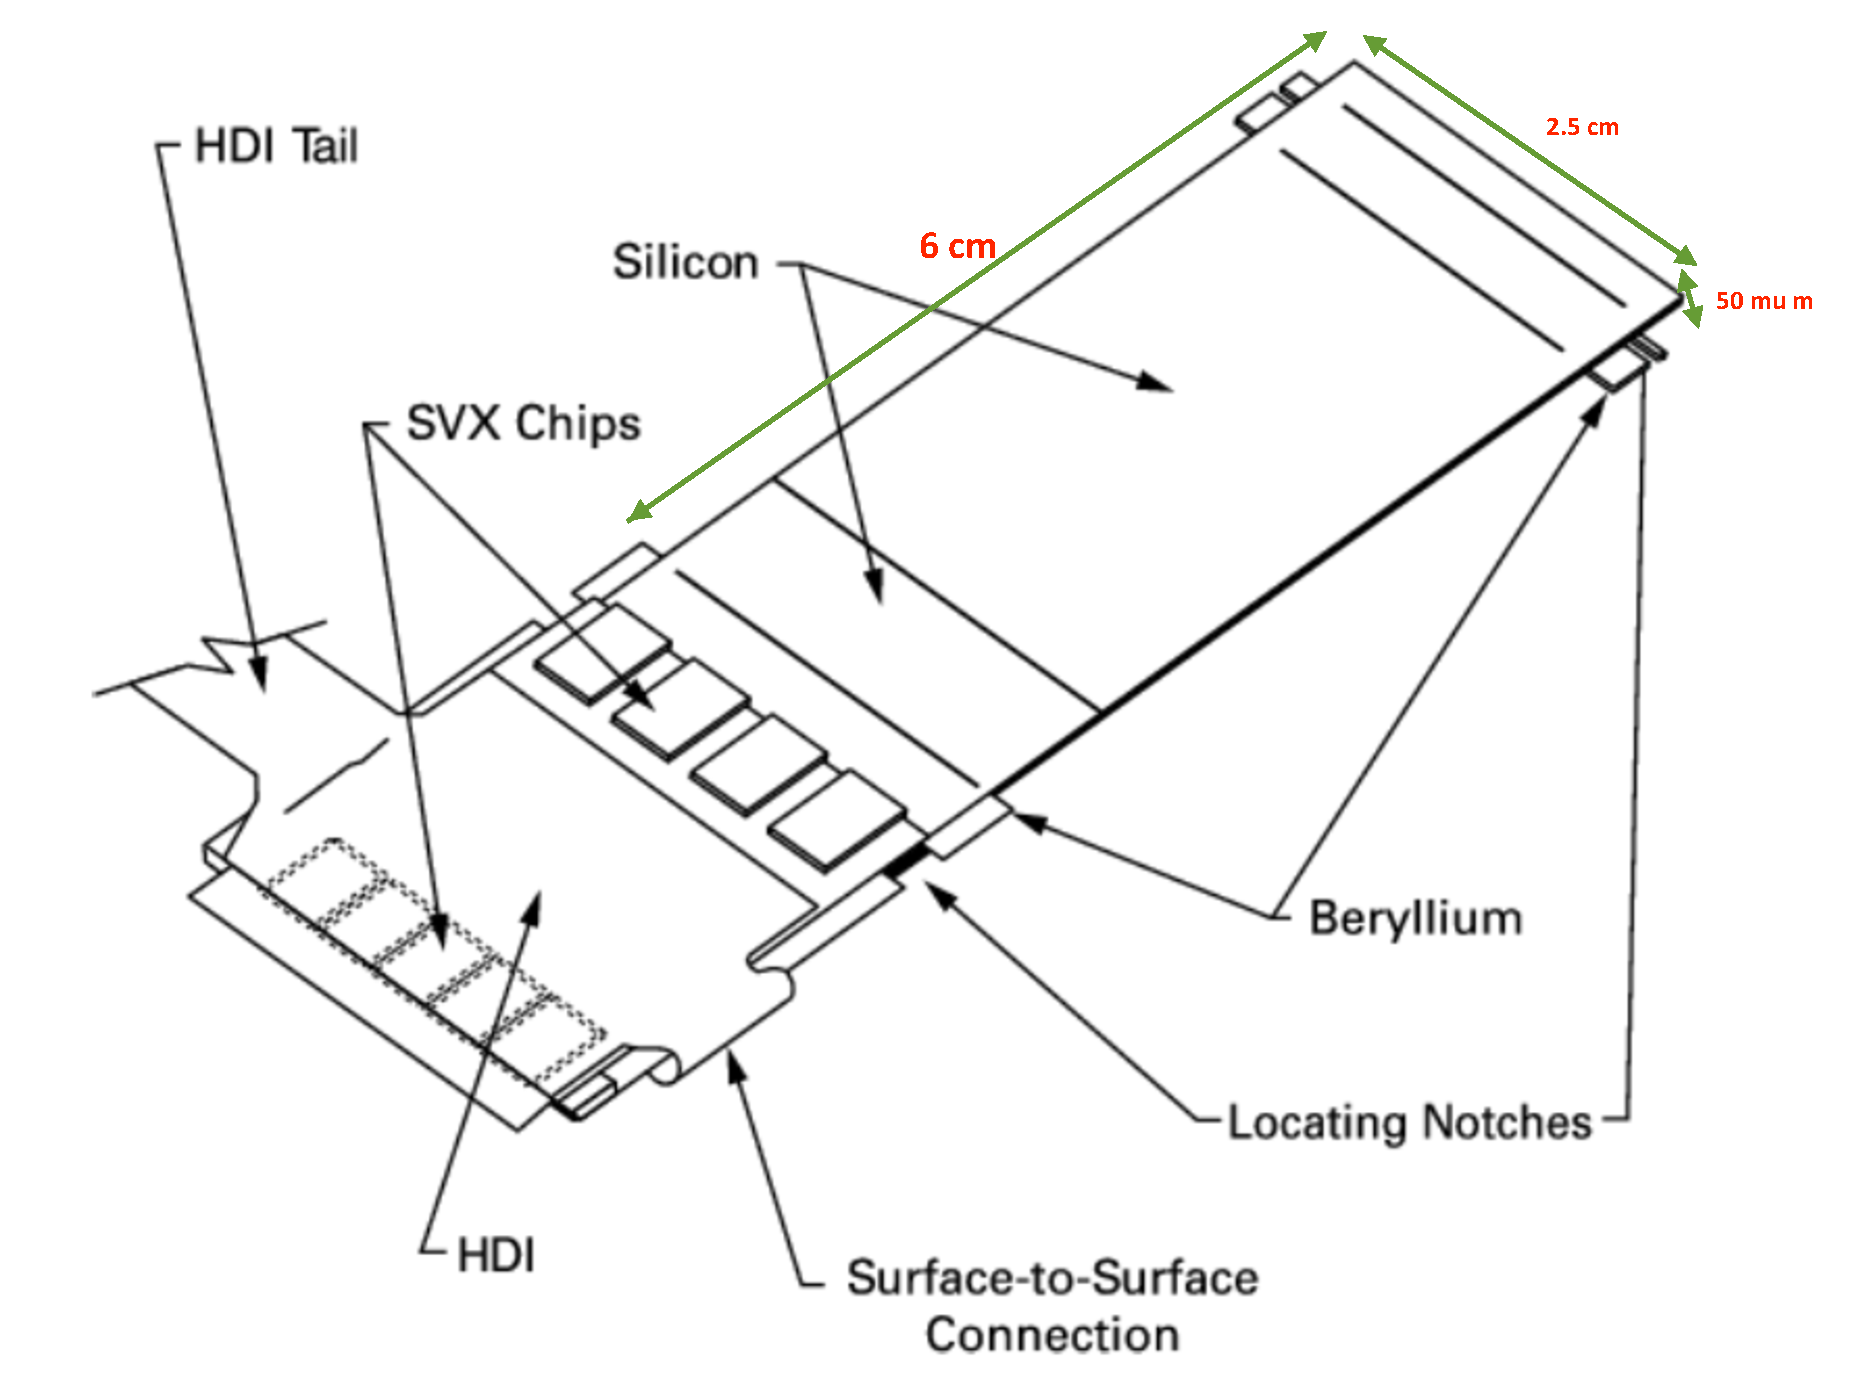
\includegraphics[height=0.3\textheight,width=0.5\textwidth]{./Images/09_SMT_03}
      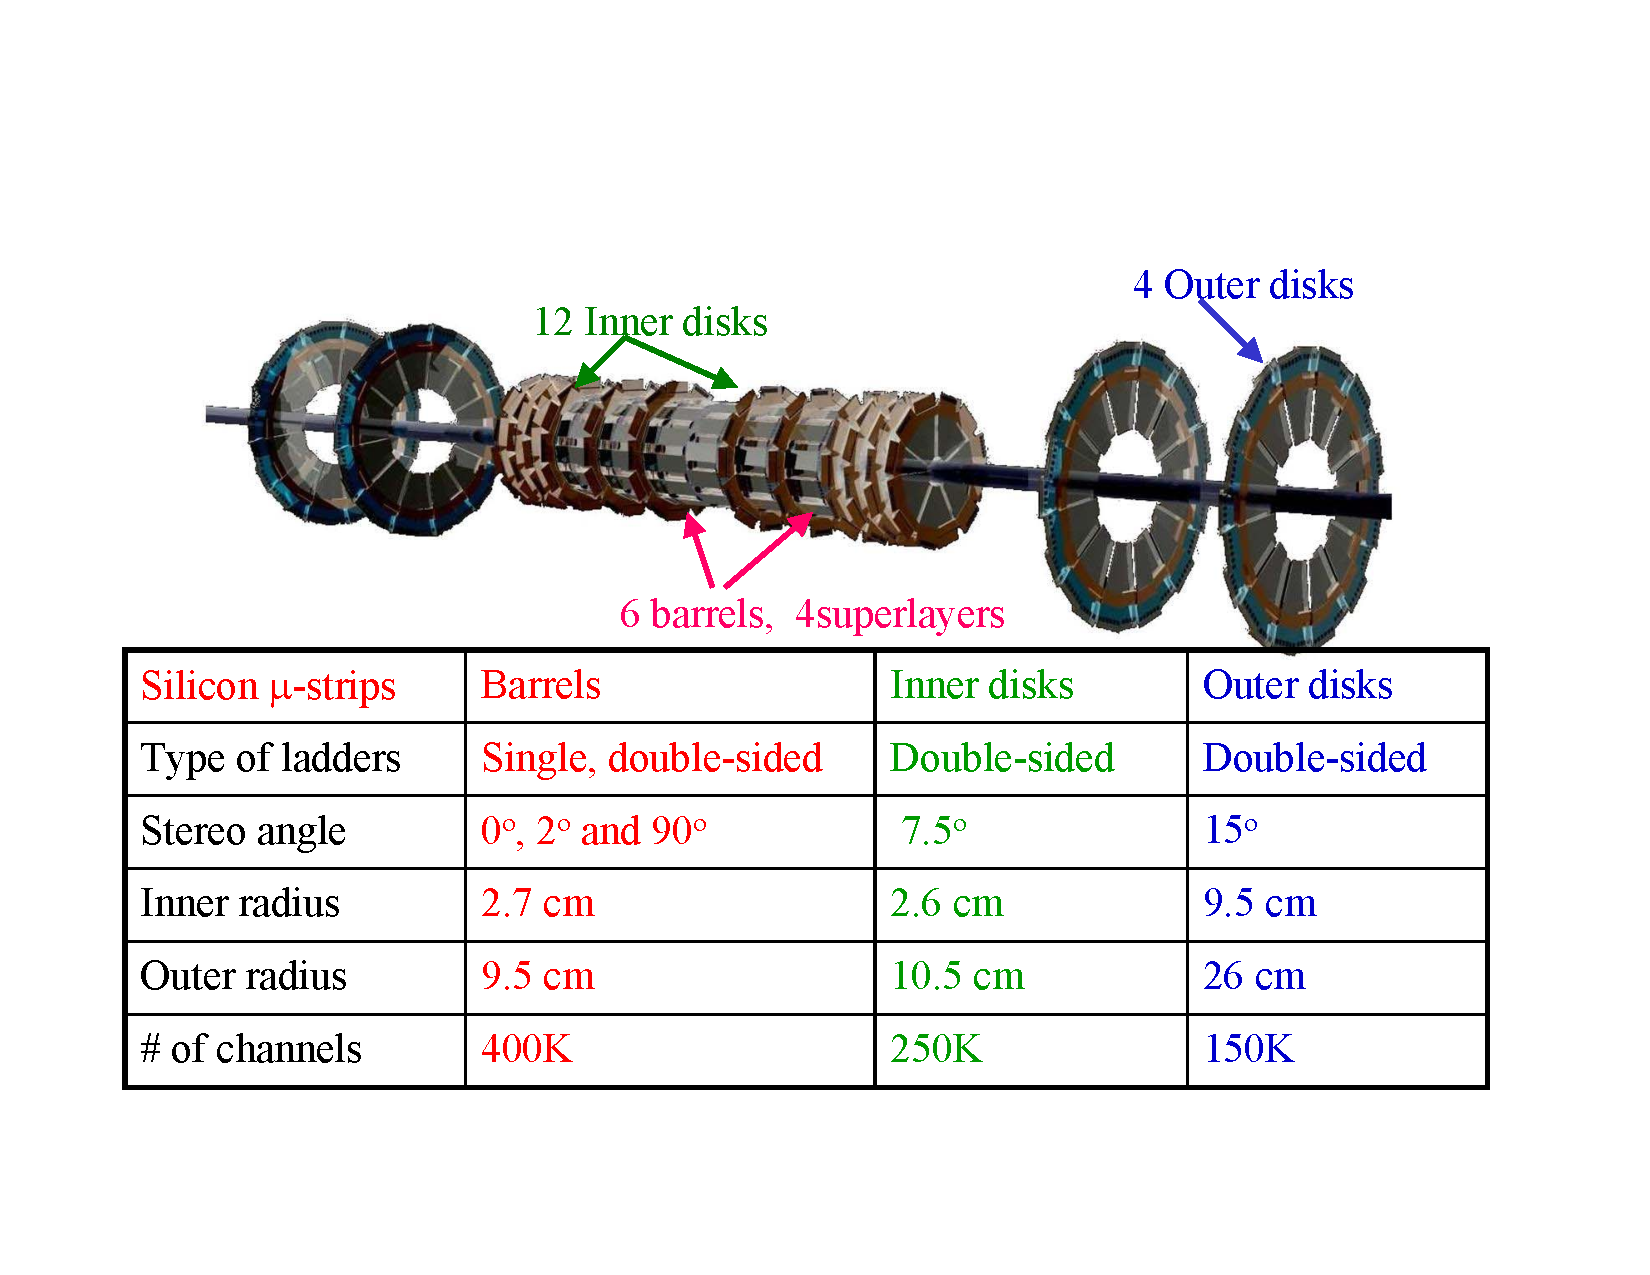
\includegraphics[height=0.3\textheight,width=0.5\textwidth]{./Images/09_SMT}
      % 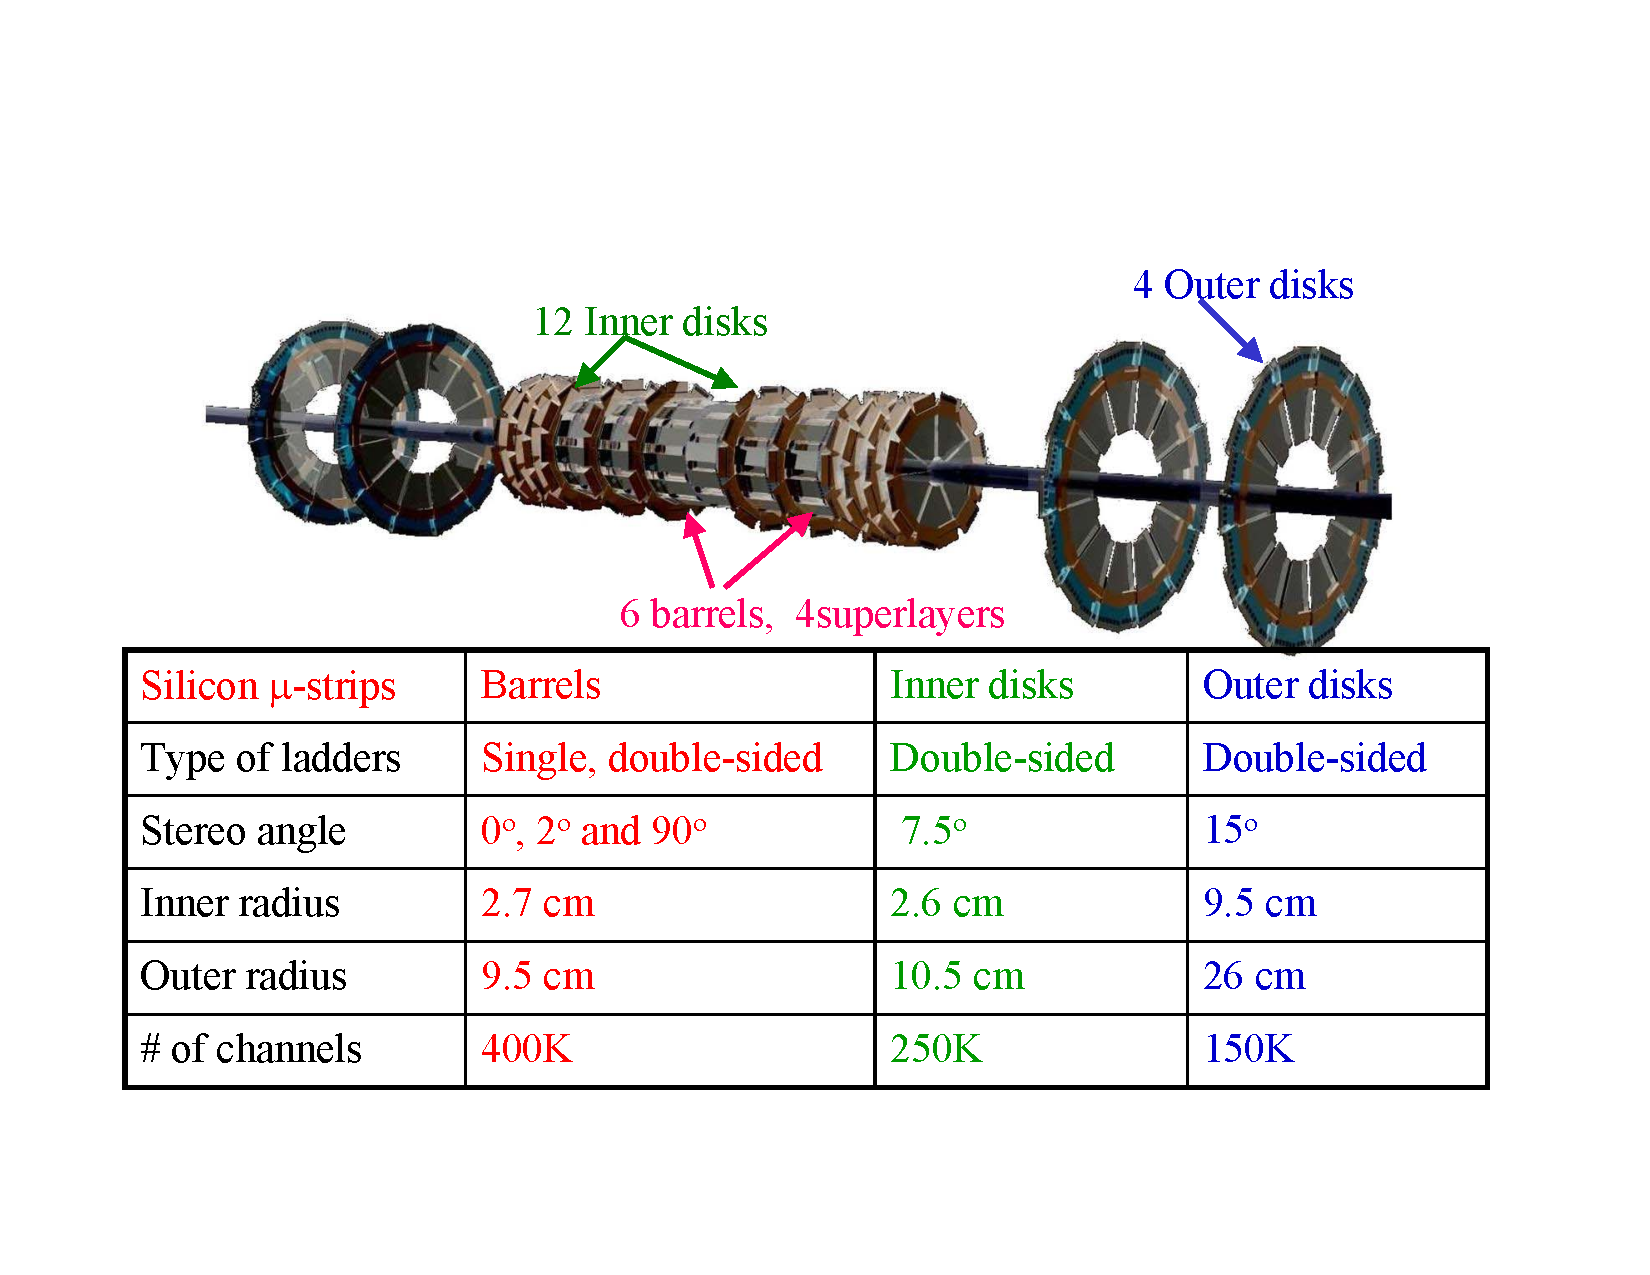
\includegraphics[height=0.3\textheight,width=0.5\textwidth]{./Images/09_SMT}
    \end{figure}
    
    \itt[<+->]
  \item The barrel gives $(r, \phi)$ coordinate and disks give $(r,
    \phi, z)$.
  \item \hlt{black}{Design considerations:}\\ minimal mass, precise
    alignment, good thermal performance and front-end electronics.
  \item \hlt{Orange}{Unit cell:}\\ rectangular beryllium substrates with $1/2$
    silicon surfaces glued to them and a laminated readout chip.
    \tti
\end{overlayarea}
\end{frame}
%%%%%% SLIDE
\begin{frame}{\textcolor{Goldenrod}{Silicon Microstrip Tracker}}
  \begin{overlayarea}{\textwidth}{\textheight}
    \begin{figure}[h]
      \centering
      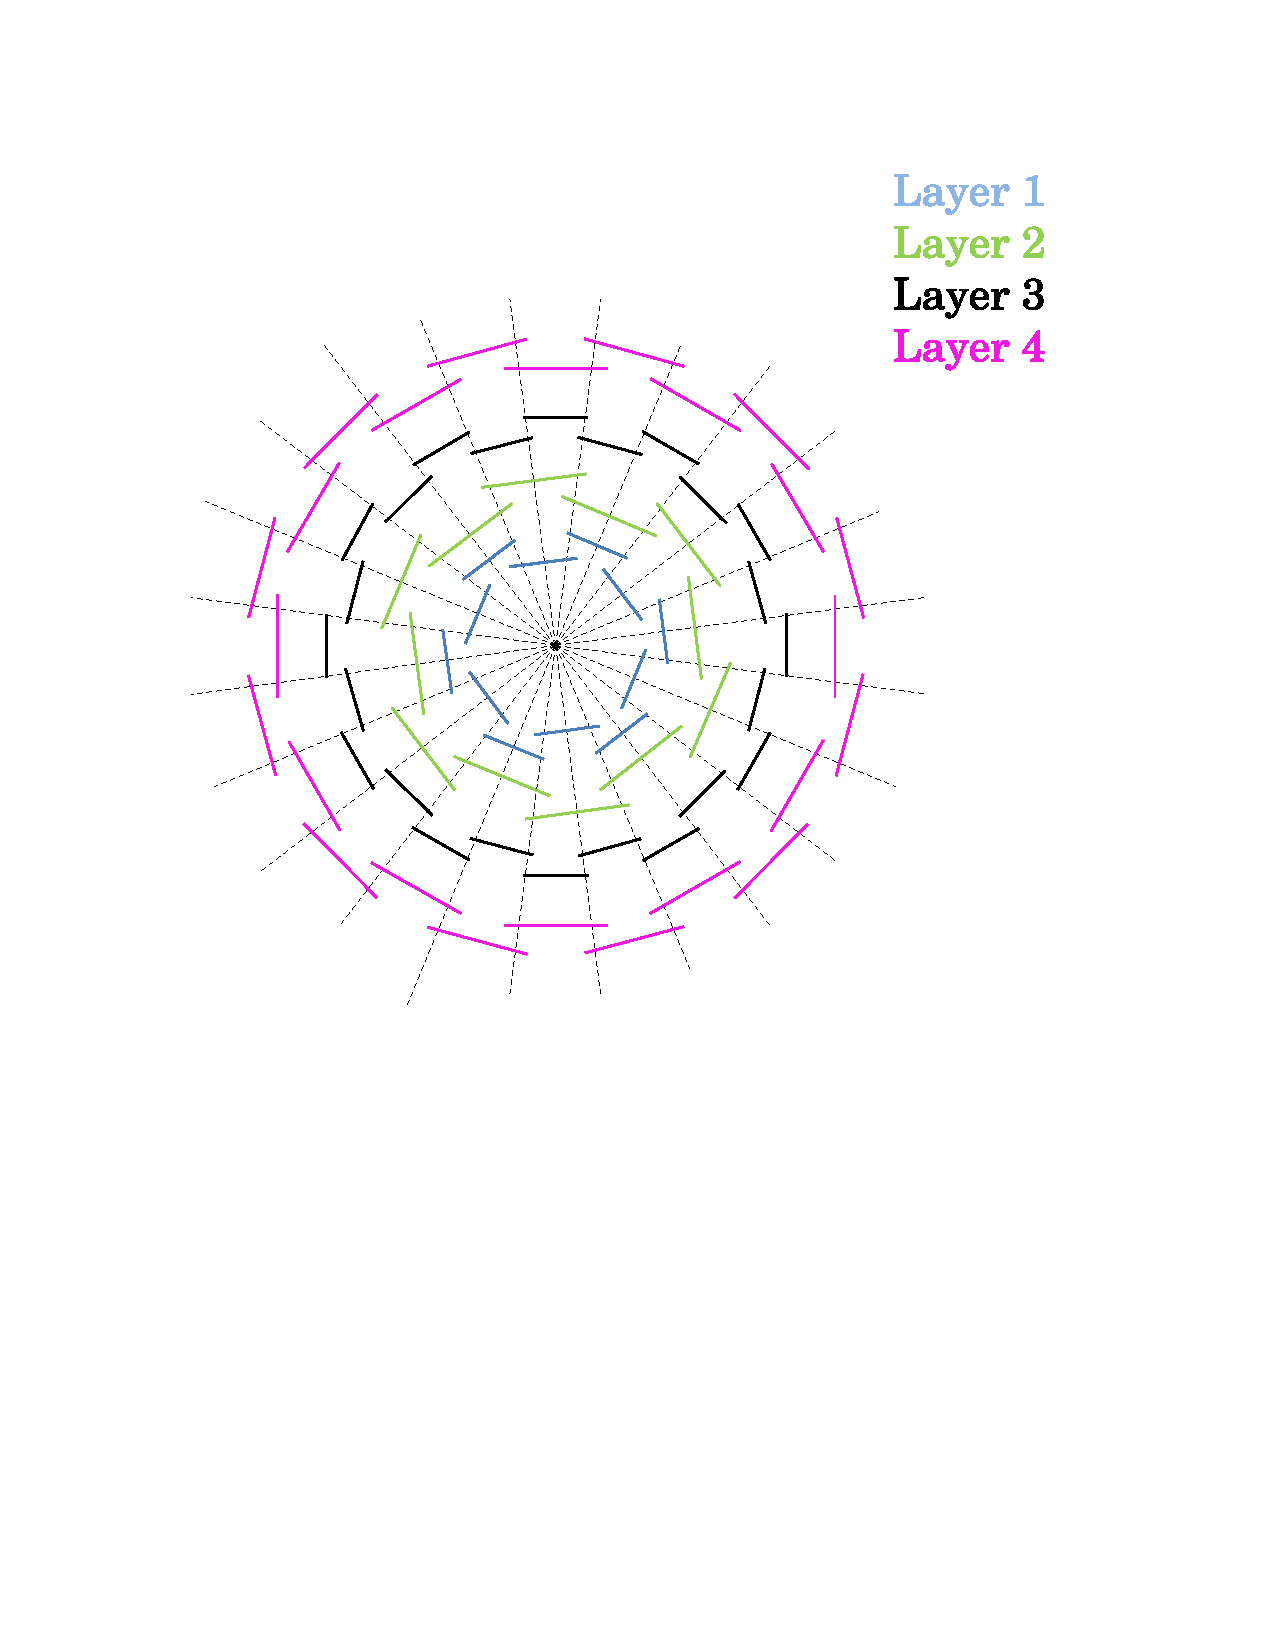
\includegraphics[height=0.34\textheight]{./Images/09_SMT_01}
      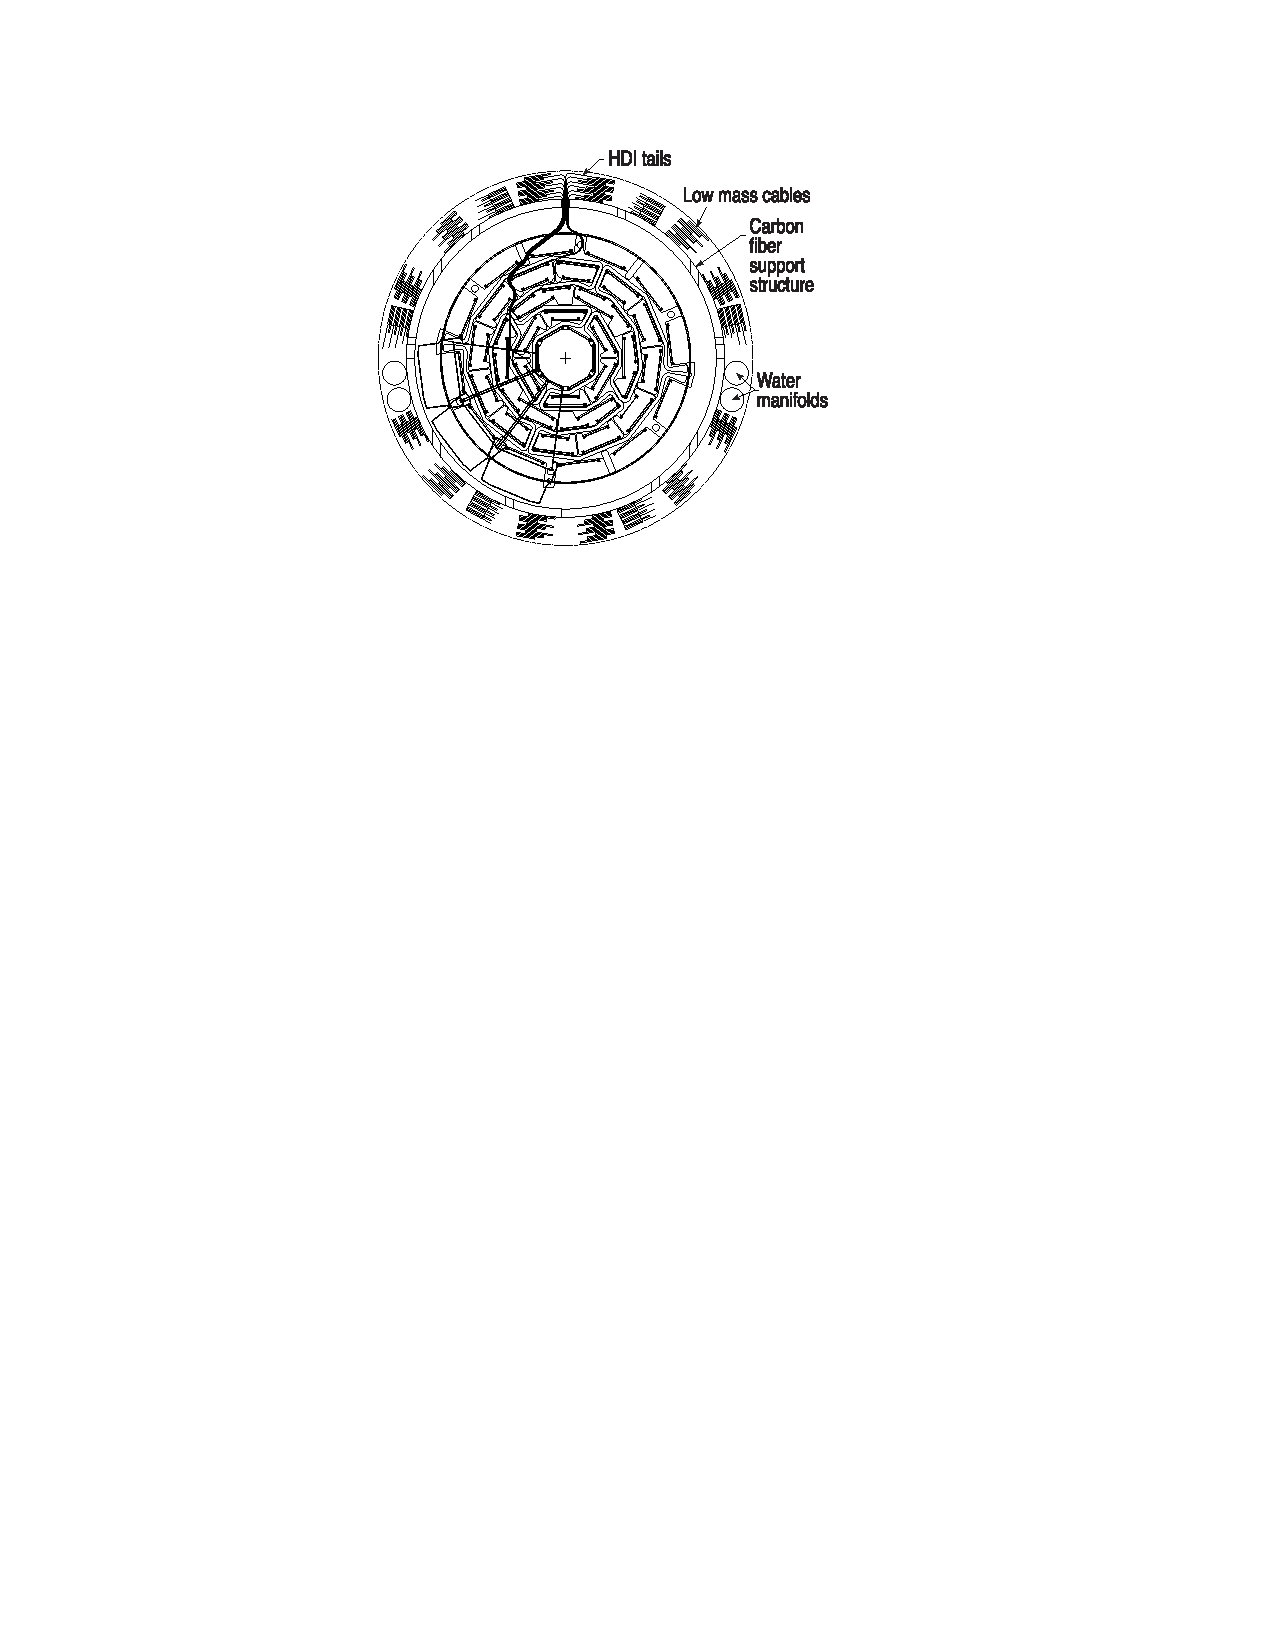
\includegraphics[height=0.34\textheight]{./Images/09_SMT_04}
      \caption*{{\small Cross section of the SMT disk/barrel module showing
            ladders mounted on the beryllium bulkhead, sample cable paths,
            three of twelve F-disk wedges, carbon fiber support structure,
            and the low-mass cable stack.}}
      \end{figure}
    \itt
    \item \textcolor{blue}{SMT support structure:\\}
      two double-walled carbon
      fiber cylinder.
    \tti
\end{overlayarea}
\end{frame}


%%%%%%%% SLIDE
\begin{frame}{\textcolor{Goldenrod}{Silicon Microstrip Tracker: Performance }}
  \begin{overlayarea}{\textwidth}{\textheight}
    \begin{figure}[h]
      \centering
      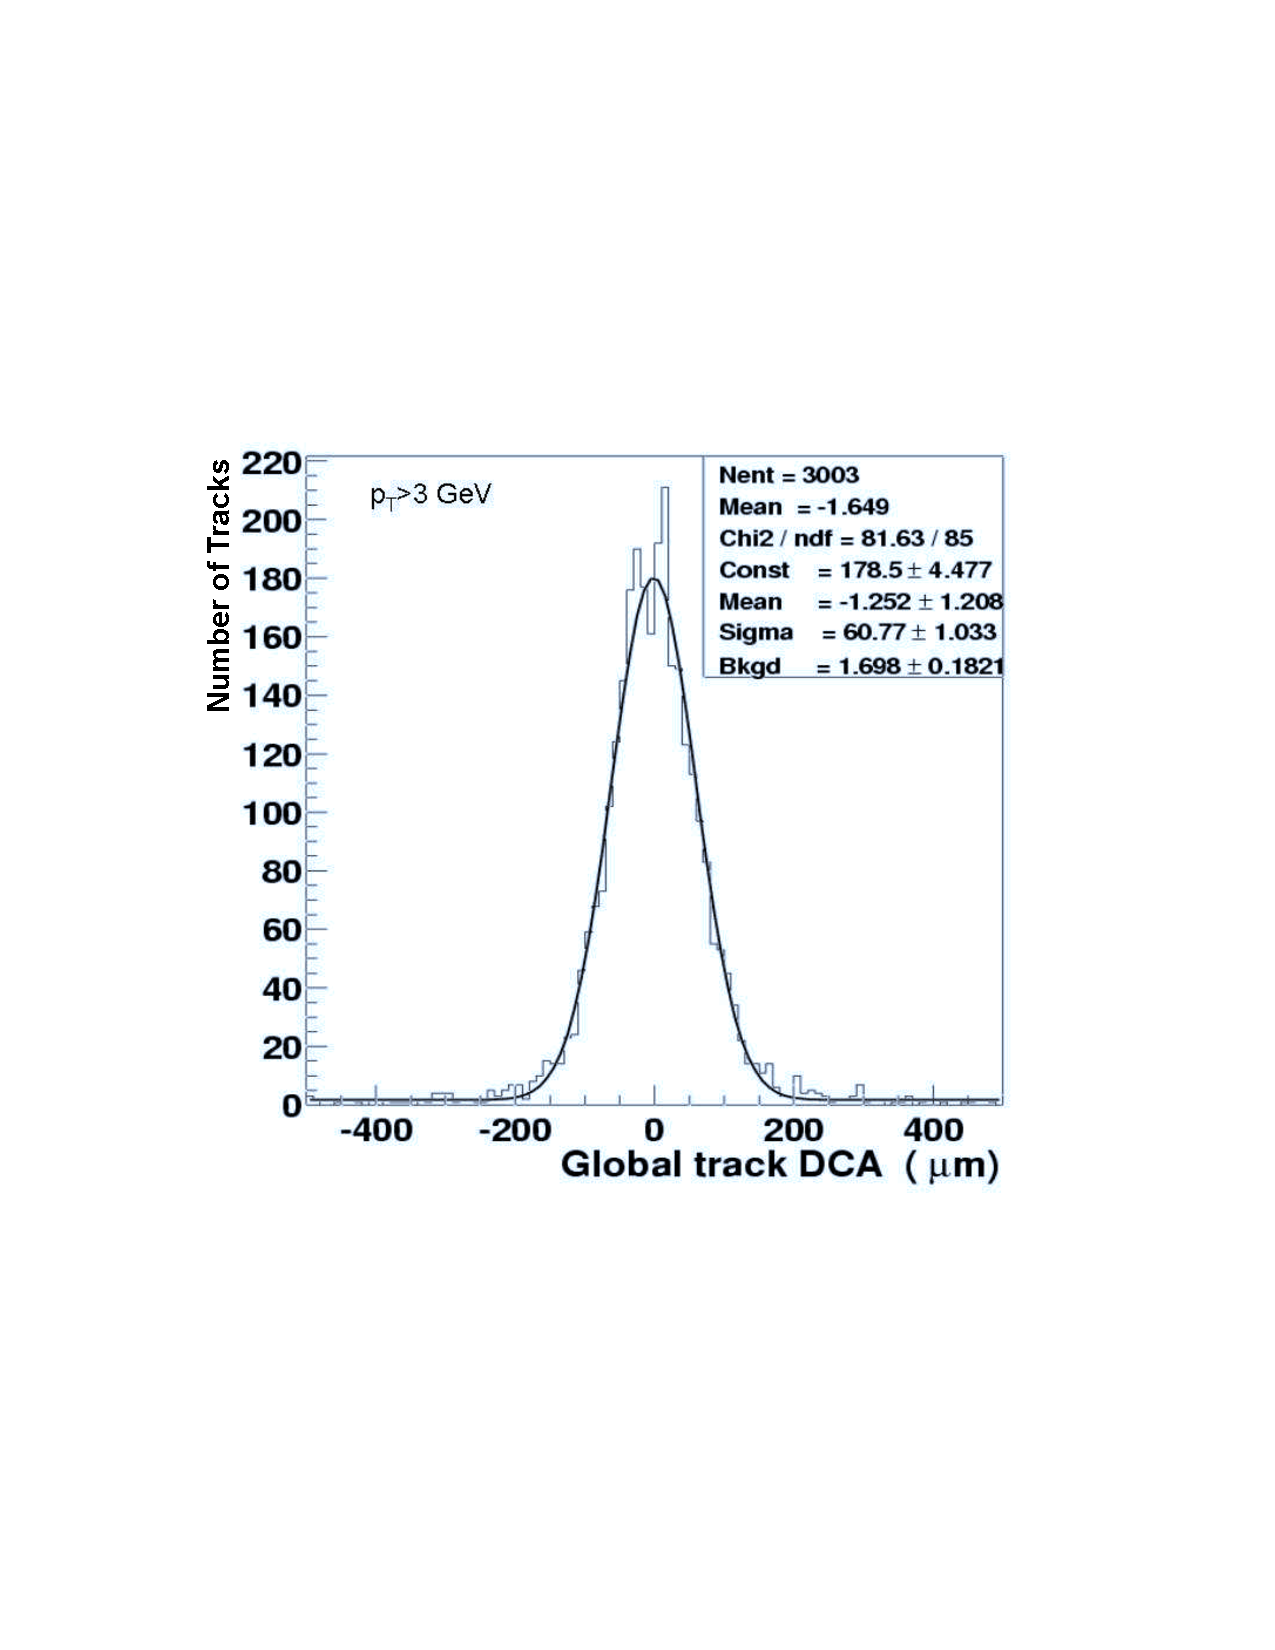
\includegraphics[height=0.35\textheight,width=0.3\textwidth]{./Images/11_SMT_01}
      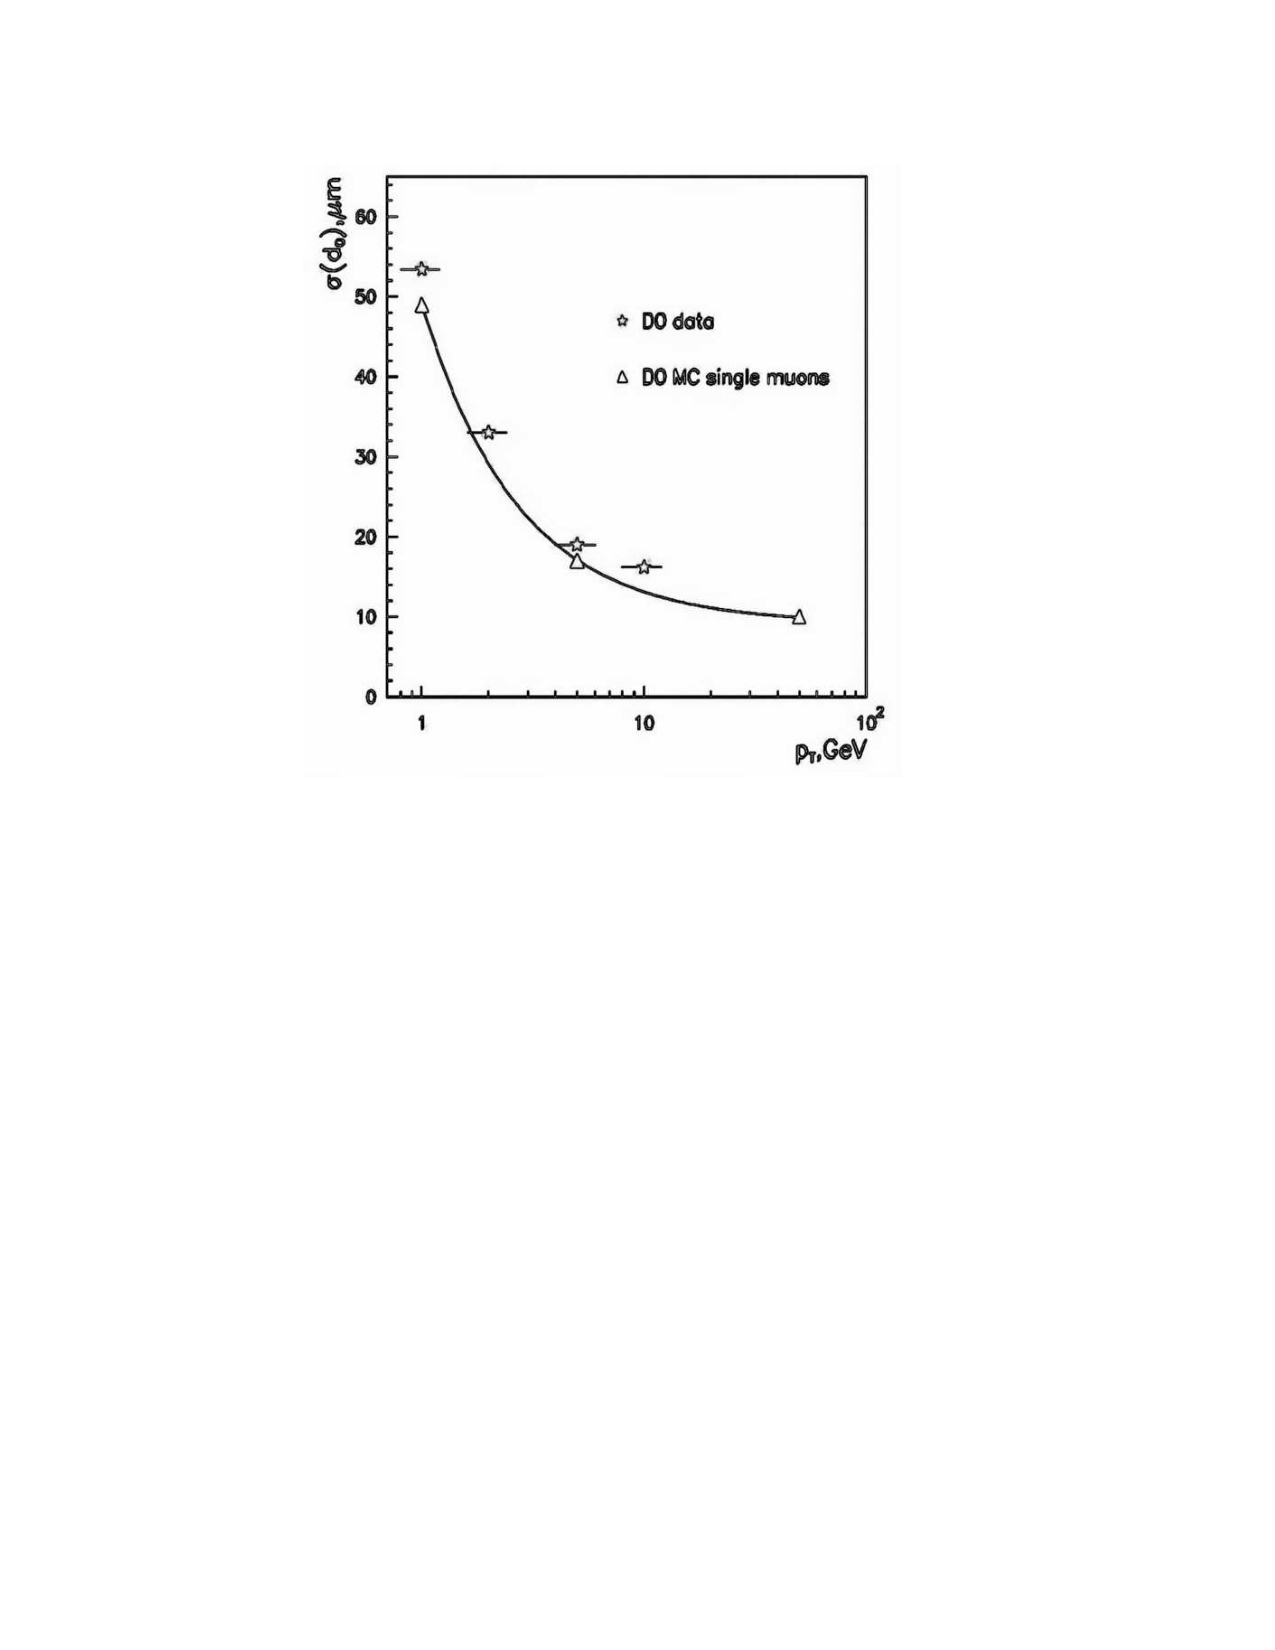
\includegraphics[height=0.35\textheight,width=0.3\textwidth]{./Images/12_SMT_01}
      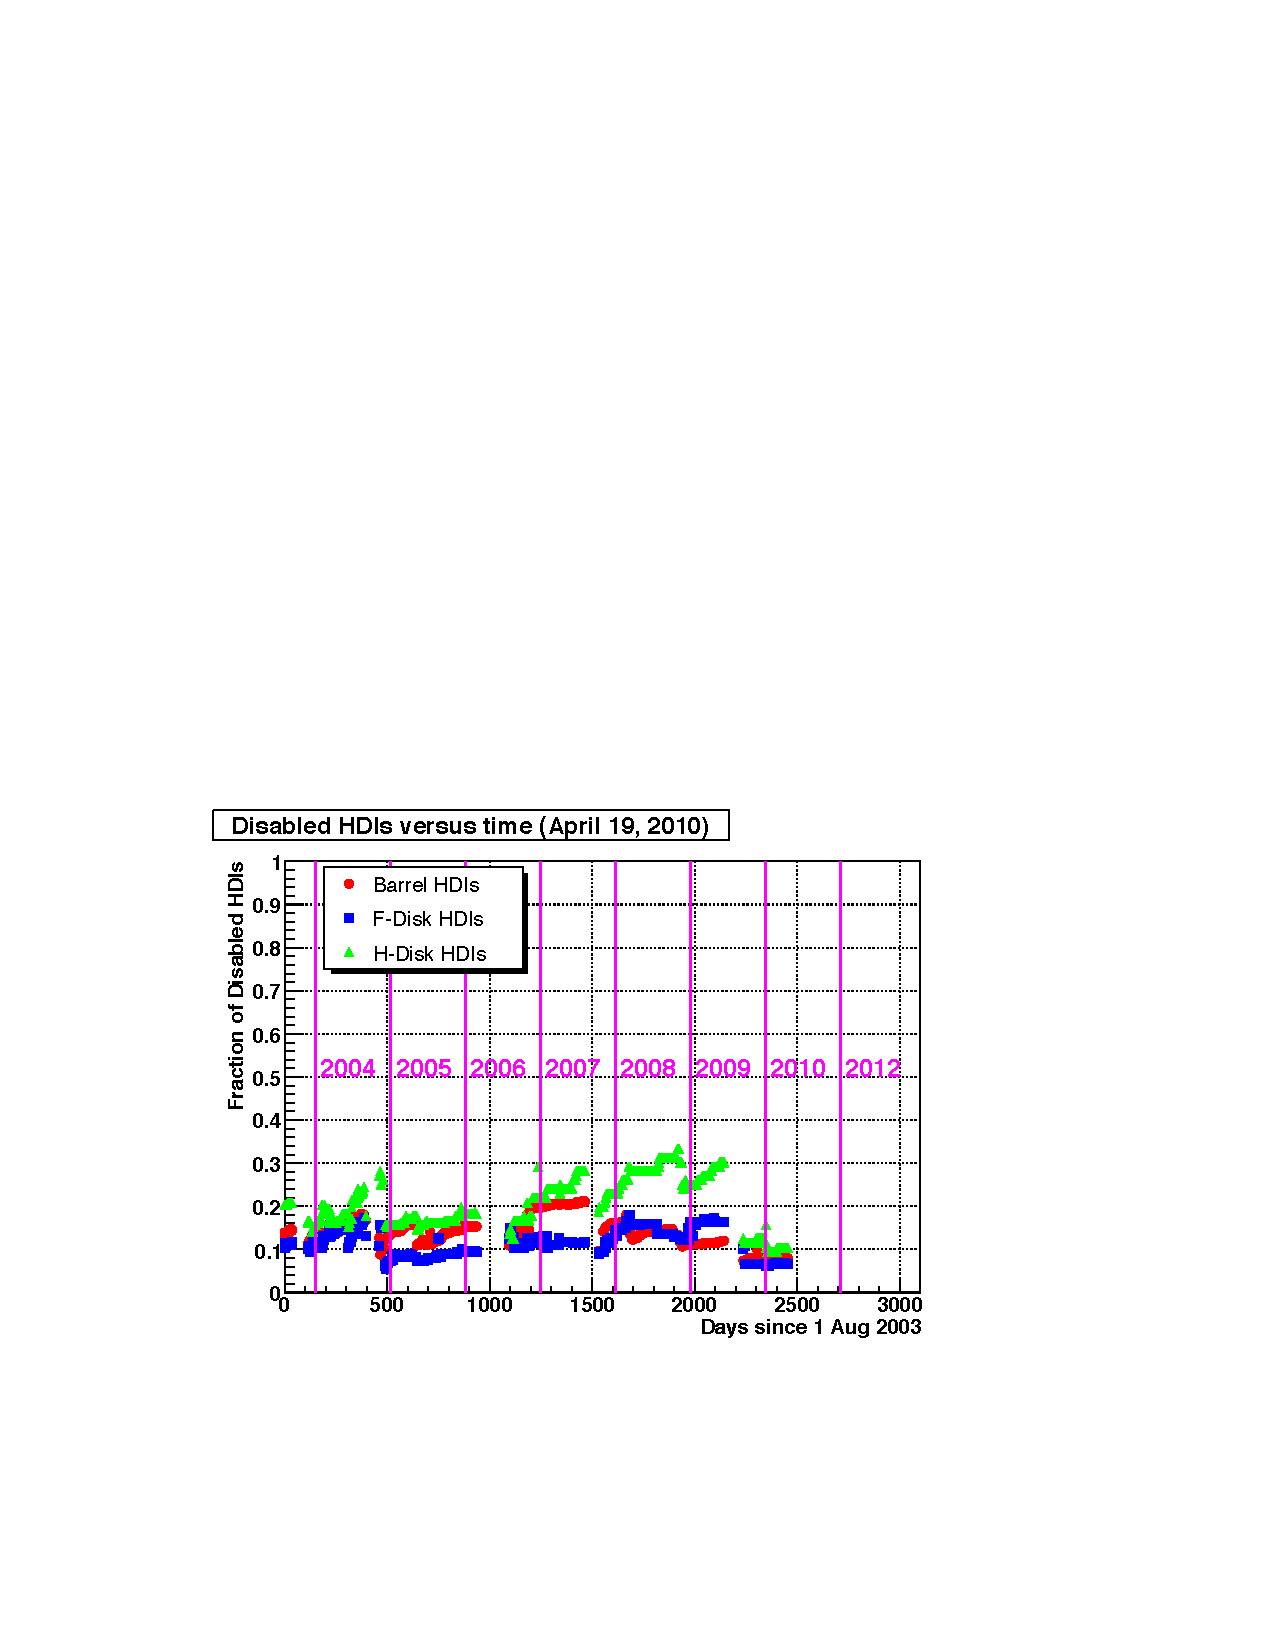
\includegraphics[height=0.35\textheight,width=0.4\textwidth]{./Images/12_SMT_02}
      
    \end{figure}
    \itt[<+->]  
  \item The signal-to-noise ratio is between $10$ and $15$
    depending on the module type
    \note{The signal is defined as the cluster
      charge given by a minimum ionizing particle including a
      correction for the incident angle, and the noise as the rms of the
      pedestal distributions.}
  \item $\sigma_{d_0} \approx 60 \mu m$ to which the beam size itself
    contributes $30$ to $40 \mu m$
  \item \alert{using both the hits in the SMT and CFT $\to$ much better
      resolution $\sigma_{d_0} \approx 15 \mu m$}
    \tti
    
% \item during run II $\approx 90$\% of sensors were functional
  
% \item most operational difficulties have been peripheral to the
%   silicon detector itself. These include latchup of operational
%   amplifiers on the interface boards, low voltage power supply
%   failures, and high leakage currents in high voltage distribution
%   boxes.
  
%   \note{\url{https://en.wikipedia.org/wiki/Latch-up}}
  
% \item the most serious detector feature is “grassy noise,”
%   which is confined to the Micron-supplied F-disk
%   detectors ($75$\% of the F-disk sensors). This noise is characterized
%   by large charge spikes which cover $10–20$ strips and
%   occur in about $20$\% of the events for affected
%   devices.
  
% \item leakage currents typically rise to
%   greater than $100 \mu A$ within one hour of turn-on at
%   the beginning of a store.
  
% \item Alignment and calibration Signal/noise performance varies with
%   detector type from $12:1 to 18:1$.
  
% \item Coherent noise is typically one-third
%   of the random noise.
  
% \item Gains vary among detector types
%   with the n-sides $5–15$\% lower than the p-sides due to the larger load
%   capacitance.
  
\end{overlayarea}
\end{frame}


\subsection{Central fiber tracker}
%%%%%% SLIDE
\begin{frame}{\textcolor{Goldenrod}{Central Fiber Tracker}}
  \begin{overlayarea}{\textwidth}{\textheight}
    \begin{figure}[h]\centering
      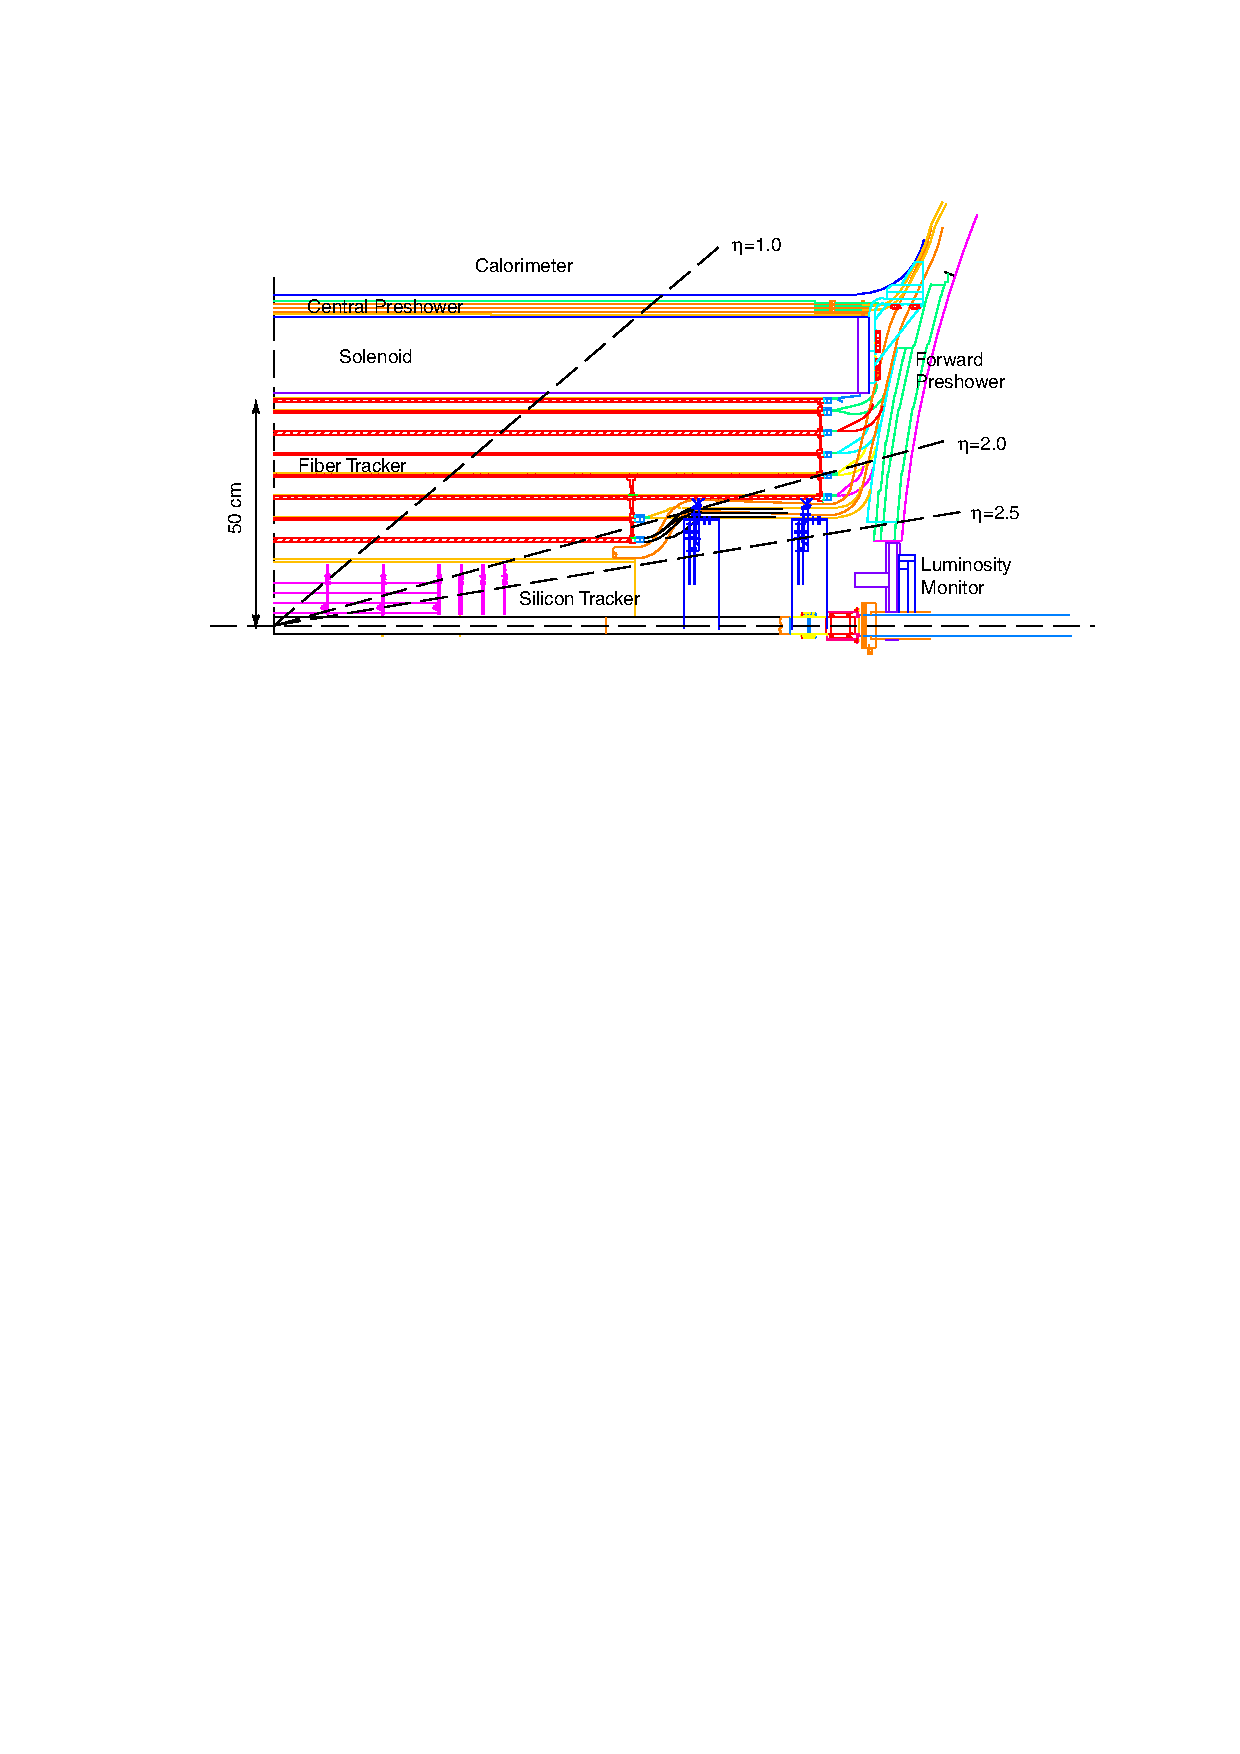
\includegraphics[height=0.4\textheight,width=0.7\textwidth]{./Images/08_CT_01.pdf}
      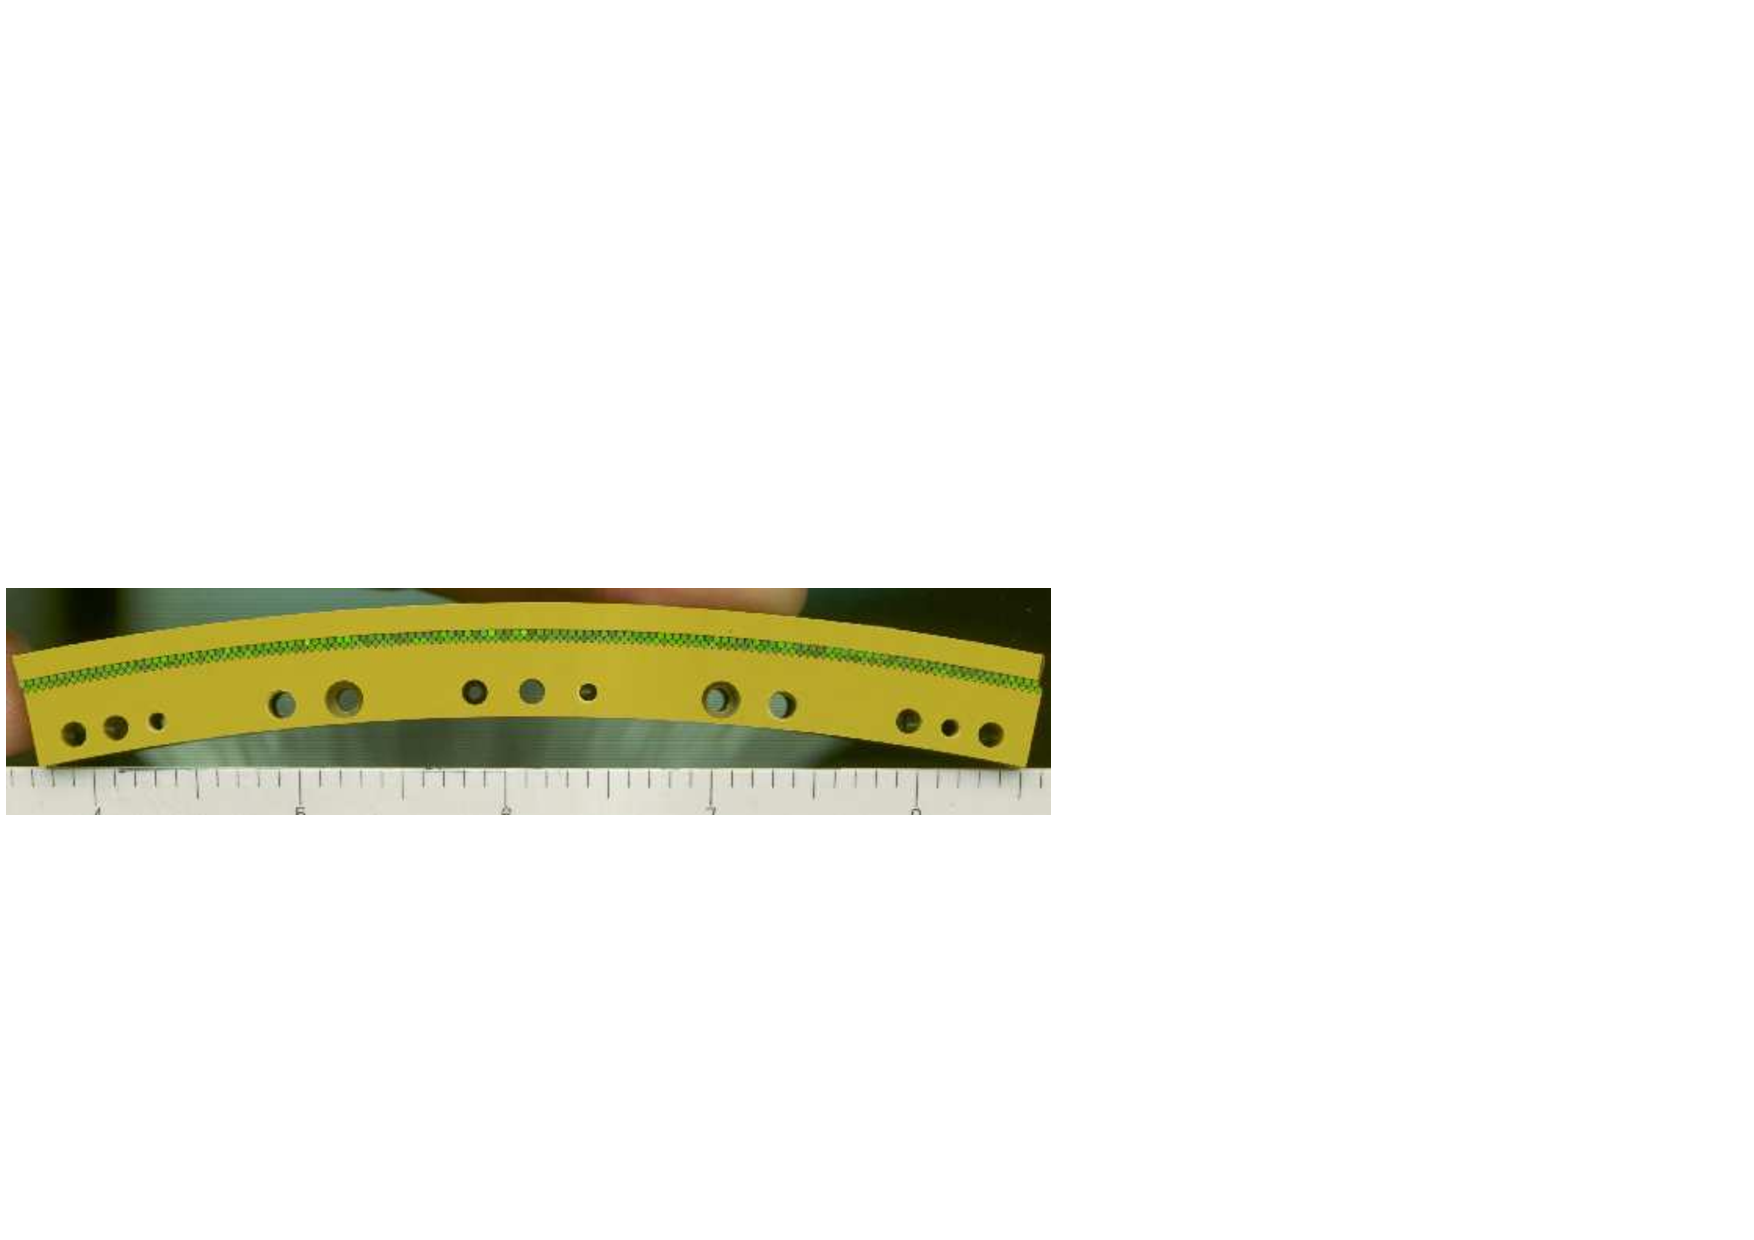
\includegraphics[height=0.1\textheight, width=0.2\textwidth]{./Images/15_CFT}
    \end{figure}
    \itt[<+->]  
    
    \note{scintillating fibers mounted on eight concentric
      support cylinders ($20 to 52 cm$ from
      the center of the beampipe. The
      two innermost cylinders are $1.66 m$ long; the outer six cylinders are
      $2.52 m$ long.}
    
    \note{ Each cylinder supports one doublet layer of fibers oriented
      along the beam direction and a second doublet layer at a
      stereo angle in $\phi$ of $+3^{\textdegree}$.}
    
  \item $76800$ fibers: made of polystyrene (PS), \it{paraterphenyl (PT) $1$\%, and
      3-hydroxyflavone (3HF)$0.15$\%}; $d = 835 \mu m \times h =1.66/2.52 m$
  \item 8 coaxial carbon cylinders, each supporting 2 doublet layers
    of fibers
    ($0^{\textdegree}$ and $\pm 3^{\textdegree}$)
    \tti
  \end{overlayarea}
\end{frame}

%%%%%% SLIDE
\begin{frame}{\textcolor{Goldenrod}{Central Fiber Tracker: VLPC}}
  \(
  \<{0.3\textwidth}
  \img{21_CFT_VLPC.jpg}\\
  %\img{21_CFT_VLPC_01.jpg}\\
  \img{21_CFT_VLPC_02.jpg}\\
  \>
  \<{0.7\textwidth}
  \itt[<+->]

  \item The fibres are connected by $7-11 m$ long optical waveguides to
    photodetectors positioned in a cryostat underneath the central
    calorimeter
  \item light collectors are Visible Light Photon Counters (VLPCs),
    which are arsenic doped silicon diodes operating at temperatures
    of $10 K$

  \item The VLPCs have quantum efficiencies of $\approx 80$\%, high gain and less
    than $0.1$\% average noise
  \item The axial fibre layers are used in the Level 1 trigger system
  \tti
  \>
  \)
\end{frame}


%%%%%% SLIDE
\begin{frame}{\textcolor{Goldenrod}{Central Fiber Tracker: performance}}
  \begin{overlayarea}{\textwidth}{\textheight}
    \begin{figure}[h]\centering
      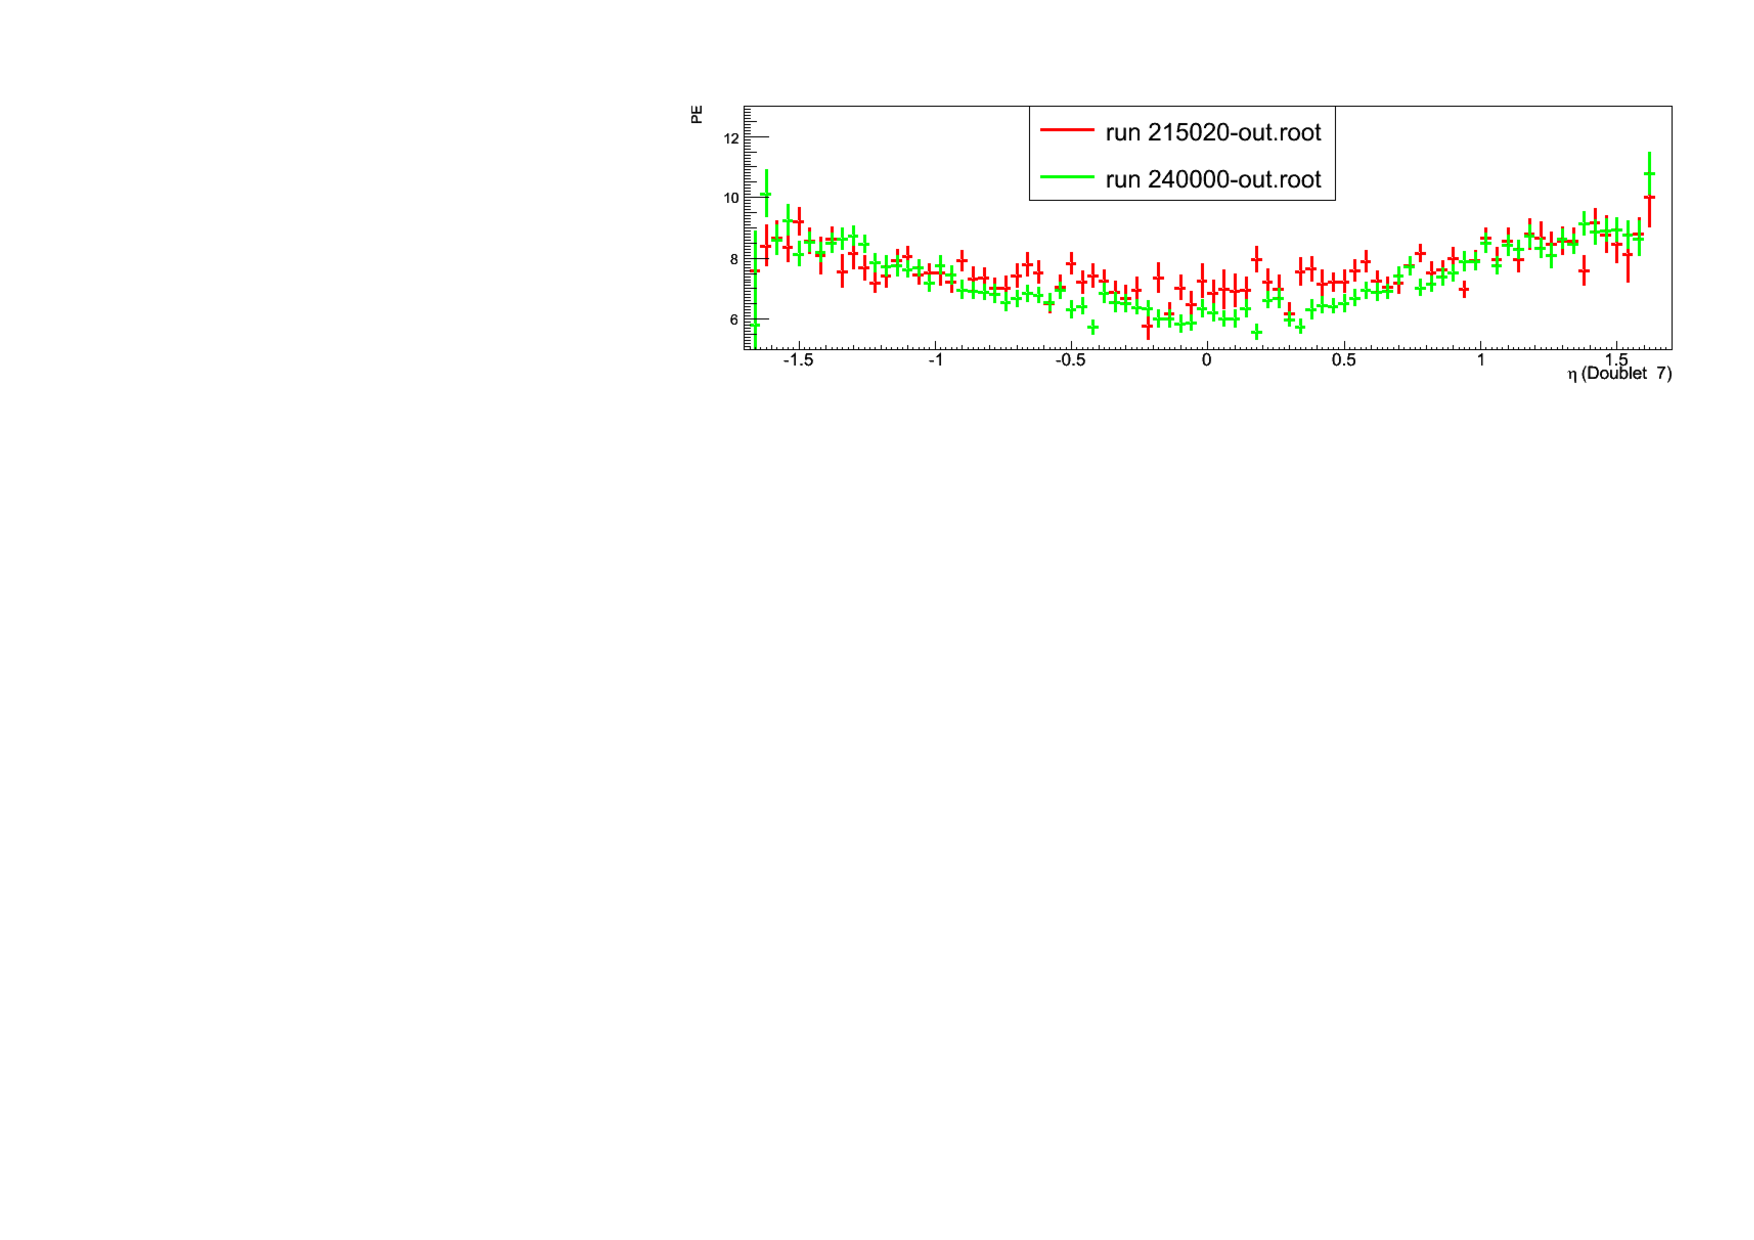
\includegraphics[height=0.2\textheight]{./Images/22_CFT_performance.pdf}\\
      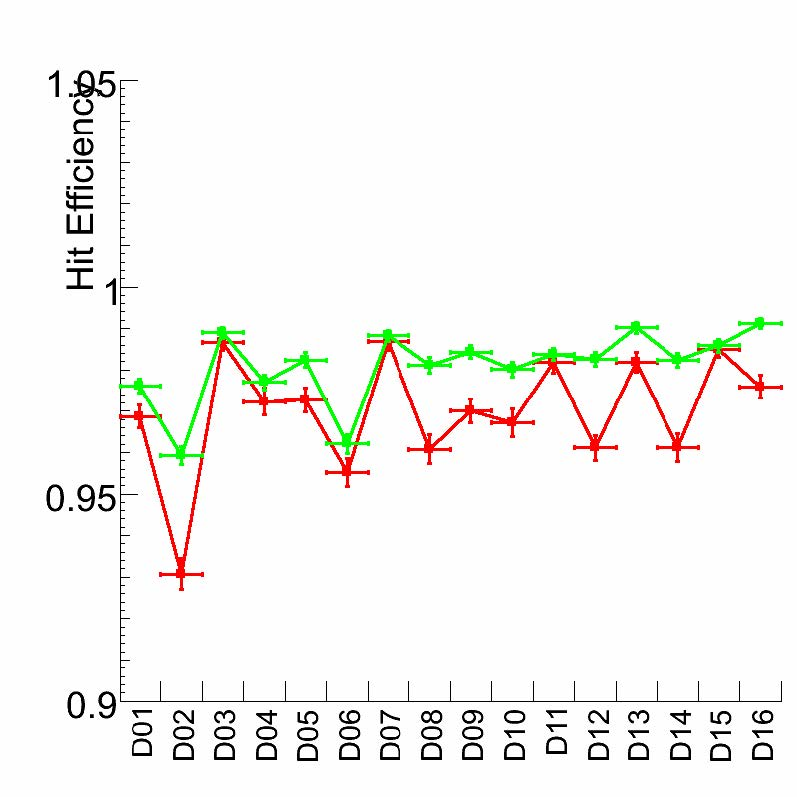
\includegraphics[height=0.3\textheight]{./Images/23_CFT_performance}
      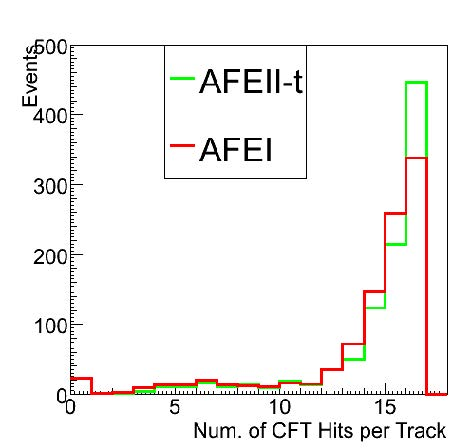
\includegraphics[height=0.3\textheight]{./Images/24_CFT_performance}
    \end{figure}
    \itt[<+->]
  \item Average photon yield depends upon path length through
    scintillator.
  \item On average 8 photons produced per hit
    \tti
 \end{overlayarea}
\end{frame}

%%%%%% SLIDE
% \begin{frame}{\textcolor{Goldenrod}{Central Fiber Tracker}}
%   \begin{overlayarea}{\textwidth}{\textheight}
%     \begin{figure}[h]\centering
      
%     \end{figure}
%     \itt[<only@+>]
    
%   \item[$\Box$] Mechanical support structure:\\
%     \itt
%   \item The eight support cylinders are each double-walled with a
%     0.25”-thick core of Rohacell [59].
    
%   \item The walls are constructed
%     from linear carbon fibers impregnated with about 40\% resin.
    
%   \item
%     Successive cylinders are nested together by thin carbon-fiber
%     annular rings that connect the inner surface of the end ring of
%     one cylinder to a carbon-fiber ring mounted on the outer fiber
%     surface of the cylinder immediately inside.
    
%   \item For tracks traversing the detector at normal incidence, the
%     thickness of each cylinder can be described as follows: 0.28\% of
%     a radiation length for the scin-
%     tillating fibers, 0.32\% for the
%     carbon fiber support cylinder, 0.13\%
%     for the glue used to make ribbons
%     out of fibers, and 0.17\% for the
%     glue used to attach the ribbons to
%     the support cylinders.
%     \tti
    
%     \tti
%   \end{overlayarea}
% \end{frame}



% %%%%%% SLIDE
% \begin{frame}{\textcolor{Goldenrod}{Central Fiber Tracker: Central Track Tigger (CTT)}}
%   \(
%   \<{0.7\textwidth}
%   \itt[<+->]
% \item Counts track candidates identified in axial view of CFT by
%   looking for hits in all 8 axial layers
% \item Combines tracking and preshower information to identify
%   electron and photon candidates
% \item
%   Generates track lists allowing other trigger systems to
%   perform track matching
%   \tti
%   \>
%   \<{0.3\textwidth}
%   \img{20_CFT}
%   \>
%   \)
% \end{frame}

